\section{Discussion}
\label{sec:discuss}
In this section, we will discuss some implementation details
and the limitations of our system. 
The medical images that we have can pose various problems 
for a traditional OCR engine to process. For example, 
the textual information on the medical images may be 
covered by grid lines as shown in \figref{fig:ecgexample2} or 
in the inverted colour. In these situations, the results of 
the OCR engine will garbled. We preprocess the 
images to remove those noises. First, we threshold the 
images and turn them into binary images. 
% Thresholding is the simplest method of image segmentation. 
Separate thresholds for each of the RGB channels of the image 
are used and combined them with an AND operation. 
In order to automatically threshold the images, 
we make use of ImageJ \cite{schneider2012671}, which implements many
existing auto-thresholding algorithms. 
Then we invert the color of the images if the text 
is white color. 
After preprocessing, we get a simplified version of the 
images and make the text on the images stand out. 
% contrast the text on the images. 
%An example of this preprocessing result is shown in \figref{fig:preprocess}. 

%\begin{figure*}[ht]
%\centering
%\subfloat[Before Preprocessing]{
%\label{fig:preprocess:1}
%\epsfig{file=figure/f1.eps, width=0.45\columnwidth}
%}
%\hfill
%\subfloat[After Preprocessing]{
%\label{fig:preprocess:2}
%\epsfig{file=figure/pref1.eps, width=0.45\columnwidth}
%}
%\caption{Results of Preprocessing}
%\label{fig:preprocess}
%\end{figure*}
%% \KZ{There seems to be some repetition from the eval section.} 
%

In our system, two parameters are important for the 
performance. 
One is the parameter $k$ in the {\em Constraint} function 
\equref{equ:constraint}, which affects the weight of 
the spatial constraints.
Another is the threshold $t$ in the same function, which 
determines whether the input data satisfy the 
type and spatial constraints based on our scoring policies 
and how many candidates will be generated.  

%\JL{In our system, two parameters which should be defined by ourselves are very important.One is the parameter $k$ in the {\em Constraint} function 
%	\equref{equ:constraint}, 
%	which affects the weight of 
%	the spatial constraints in the whole set of constraints. Another is the threshold we set since an appropriate threshold could give us appropriate numbers of candidates after the selection by filtering some bad results.}
% \KZ{Which param in constraint. The constraint function needs to be
% defined carefully.}
In the implementation process, 
we hold out 20 images separately to train these two parameters 
and choose the ones that have the best performance. 
% some more results

Although our system achieves good results based on our 
experiments, there are some limitations that call for future 
work. First, in order to fuzzy match the information onto the images, 
we need to provide enough constraints in the description, 
such as the type of the 
data or the range of the data. If the constraints are not 
sufficiently specified, it is hard for our system to evaluate what 
data among the OCR outputs are more suitable for the description. 
For example, if we constrain the data to be an integer in the 
description, then any integers that appear in the OCR output can be 
candidates if they satisfy the spatial constraints. 
In many cases, insufficiency in the constraints can be 
made up by the constraints indicated from the neighboring descriptions. 
But sometimes, simple descriptions will lead to sub-standard results. 
Second, the correction model 
we generated is a probabilistic model based on the statistics. 
This correction model can make mistakes, 
e.g., correcting the right answer into the wrong one. More data 
from manual correction will help to reduce this possibility. 

% \KZ{Perhaps there's more issues you can discuss, now that u have
% changed the def of the correction model...}
